\documentclass[11pt]{article}

% This file will be kept up-to-date at the following GitHub repository:
%
% https://github.com/automl-conf/LatexTemplate
%
% Please file any issues/bug reports, etc. you may have at:
%
% https://github.com/automl-conf/LatexTemplate/issues

\usepackage{microtype} % microtypography
\usepackage{booktabs}  % tables
\usepackage{url}  % urls

% AMS math
\usepackage{amsmath}
\usepackage{amsthm}

% With no package options, the submission will be anonymized, the supplemental
% material will be suppressed, and line numbers will be added to the manuscript.
%
% To hide the supplementary material (e.g., for the first submission deadline),
% use the [hidesupplement] option:
%
% \usepackage[hidesupplement]{automl}
%
% To compile a non-anonymized camera-ready version, add the [final] option (for
% the main track), or the [finalworkshop] option (for the workshop track), e.g.,
%
% \usepackage[final]{automl}
% \usepackage[finalworkshop]{automl}
%
% or
%
% \usepackage[final, hidesupplement]{automl}
% \usepackage[finalworkshop, hidesupplement]{automl}

\usepackage[final]{automl}

% You may use any reference style as long as you are consistent throughout the
% document. As a default we suggest author--year citations; for bibtex and
% natbib you may use:

\usepackage{natbib}
\bibliographystyle{apalike}

% and for biber and biblatex you may use:

% \usepackage[%
%   backend=biber,
%   style=authoryear-comp,
%   sortcites=true,
%   natbib=true,
%   giveninits=true,
%   maxcitenames=2,
%   doi=false,
%   url=true,
%   isbn=false,
%   dashed=false
% ]{biblatex}
% \addbibresource{...}

% Own packages
\usepackage{hyperref}
\hypersetup{
    colorlinks=true,
    linkcolor=blue,
    filecolor=magenta,      
    urlcolor=cyan,
    pdftitle={Overleaf Example},
    pdfpagemode=FullScreen,
    }
\usepackage{float}
\usepackage{adjustbox}
\usepackage{longtable}
\usepackage{tabularx}
\usepackage{caption}
\usepackage{rotating}

\title{Example Submission Final Project AutoML Lecture WS 2022/2023}

% The syntax for adding an author is
%
% \author[i]{\nameemail{author name}{author email}}
%
% where i is an affiliation counter. Authors may have
% multiple affiliations; e.g.:
%
% \author[1,2]{\nameemail{Anonymous}{anonymous@example.com}}

\author[1]{\nameemail{Constantin von Crailsheim}{C.Crailsheim@campus.lmu.de}}

% the list might continue:
% \author[2,3]{\nameemail{Author 2}{email2@example.com}}
% \author[3]{\nameemail{Author 3}{email3@example.com}}
% \author[4]{\nameemail{Author 4}{email4@example.com}}

% if you need to force a linebreak in the author list, prepend an \author entry
% with \\:

% \author[3]{\\\nameemail{Author 5}{email5@example.com}}

% Specify corresponding affiliations after authors, referring to counter used in
% \author:

\affil[1]{LMU Munich, Institute of Statistics}

% the list might continue:
% \affil[2]{Institution 2}
% \affil[3]{Institution 3}
% \affil[4]{Institution 4}

% define PDF metadata, please fill in to aid in accessibility of the resulting PDF
\hypersetup{%
  pdfauthor={}, % will be reset to "Anonymous" unless the "final" package option is given
  pdftitle={},
  pdfsubject={},
  pdfkeywords={}
}

\begin{document}

\maketitle

\begin{abstract}
\end{abstract}

% content will be automatically hidden during submission
% \begin{acknowledgements}

% \end{acknowledgements}

\section{Introduction}

The AutoML system should be able to deal with missing values and yield good performance as measured by the balanced accuracy on imbalanced datasets. Thus, it optimizes a ML pipeline consisting of five elements. First, a choice of two imputers replaces missing values. Then, an optional sampling method is applied to deal with imbalance in the targets, which consists of both under- and oversampling methods. Next, the pre-processed integer features are rounded such that they do not take values that would not appear in the training data. After optionally normalizing all features, three different models were fitted, i.e., a random forest classifier, a gradient boosting classifier and a SVM classifier. The choice of pre-processing and the hyperparameters of the model were optimized by DEHB, which is a computationally cheap optimizer that works well on discrete search spaces. The final predictions are derived by majority voting of the individual predictions of the best pipelines for each model. This means that the overall predictions should be good of the errors of the model are not too correlated.   

\section{Method}

This section outlines the specific choices of the AutoML system and how it will be optimized and evaluated. The choices of the imputation strategy of sklearn.impute are:
\begin{itemize}
\item The \href{https://scikit-learn.org/stable/modules/generated/sklearn.impute.SimpleImputer.html}{SimpleImputer} is an univariate imputer, which completes missing values with a descriptive statistic per feature. I chose the median, since it is less sensitive to outliers than the mean.
\item The \href{https://scikit-learn.org/stable/modules/generated/sklearn.impute.KNNImputer.html#sklearn.impute.KNNImputer}{KNNImputer} replaces missing values by the mean value of its 5 nearest neighbors as default based on Euclidian distance of their non-missing observations of the same feature. 
\end{itemize}

The choices of data-level sampling method to yield balanced dataset of imblearn are:
\begin{itemize}
\item \href{https://imbalanced-learn.org/stable/references/generated/imblearn.over_sampling.SMOTE.html}{SMOTE} as an oversampling approach generates new samples of the minority class by interpolating between existing observations of the minority class, where no distinction is made between easy and hard samples. 
\item \href{https://imbalanced-learn.org/stable/references/generated/imblearn.under_sampling.TomekLinks.html}{TomekLinks} as an undersampling approach removes samples from the majority class, if they are nearest neighbors to a minority class sample, thus removing noisy borderline samples of the majority class. 
\item \href{https://imbalanced-learn.org/stable/references/generated/imblearn.combine.SMOTETomek.html}{SMOTETomek}, which combines SMOTE and Tomek links.
\item No sampling method, which would allow algorithmic-level methods to deal with the imbalanced data. 
\end{itemize}

The above pre-processing methods could generate numeric values for features that should contain only integers (e.g., ordinal categorical features), since they impute missing values by means or medians and generate new samples by interpolation. Thus, another layer is added to the pipeline, which rounds all observations of those features to an integer. \\

The last step of pre-processing is  the choice of whether to apply the \href{https://scikit-learn.org/stable/modules/generated/sklearn.preprocessing.StandardScaler.html}{StandardScaler} of sklearn.preprocessing to standardize the features. This will be in particular useful for the SVM, since an RBF kernel assumes features centered around zero and similar variance across features. \\

Subsequently, the hyperparameters of the three models of the ensemble were optimized, where the search space was defined with the \href{https://automl.github.io/ConfigSpace/main/}{ConfigSpace} package. For almost all hyperparameters, the default was set to the default specified for each model. The search space was mostly chosen such that it is centered around the default while accounting for log scale. In those cases where the default would be a the lower end of a reasonable search space, the upper bound was chosen higher. \\

The first model in the ensemble is a \href{https://scikit-learn.org/stable/modules/generated/sklearn.ensemble.RandomForestClassifier.html}{RandomForestClassifier} from sklearn.ensemble. It can handle all data types well and generalizes well by having a low variance due to ensembling over relatively uncorrelated models. The hyperparameters, which will all be sampled uniformly, are:

\vspace{-0.3cm}
\begin{table}[h]
\begin{tabular}{ | c | c | c | c | c | c | }
 \hline
  Hyperparameter & Data type & Search space & Default & Other \\
 \hline
 criterion & Categorical & \{Gini, Entropy, Log loss\} & Gini &   \\ 
 max\_depth  & Integer & [5,15] & 10 &  \\ 
 min\_samples\_split & Integer & [1, 32] & 2 & Log scale \\ 
 min\_samples\_leaf & Integer & [1, 16] & 1 & Log scale  \\ 
 max\_features & Integer & [0.1, 0.9] & 0.5 &   \\  
 class\_weight & Categorical & \{Balanced, Balanced subsample, None\}  & None &  \\ 
 \hline
\end{tabular}
\end{table}
\vspace{-0.3cm}

The class\_weight is an algorithm-level method that deals with imbalanced data and will only have an effect if no data-level sampling method was used, since in that case the dataset passed to the model will be balanced. \\

The second model in the stack is a \href{https://scikit-learn.org/stable/modules/generated/sklearn.ensemble.GradientBoostingClassifier.html}{GradientBoostingClassifier} from sklearn.ensemble. It has strong predictive performance by iteratively fitting weak learners on the error of the previous learner and has similar advantages as the RandomForestClassifier. The hyperparameters are:

\vspace{-0.3cm}
\begin{table}[h]
\begin{tabular}{ | c | c | c | c | c | c | }
 \hline
  Hyperparameter & Data type & Search space & Default & Other \\
 \hline
 loss & Categorical & \{Log loss, Exponential\} & Log loss &  \\ 
 learning\_rate & Float & [0.01, 1] & 0.1 & Log scale  \\ 
 criterion & Categorical & \{Friedman MSE, Squared error\} & Friedman MSE &   \\ 
 min\_samples\_split & Integer & [1, 32] & 2 & Log scale \\ 
 min\_samples\_leaf & Integer & [1, 16] & 1 & Log scale  \\
 max\_depth  & Integer & [2,10] & 3 &  \\ 
 \hline
\end{tabular}
\end{table}
\vspace{-0.3cm}

The third model in the stack is a Support Vector Classifier (\href{https://scikit-learn.org/stable/modules/generated/sklearn.svm.SVC.html#sklearn.svm.SVC}{SVC}) from sklearn.svm. This model works in particular well on easily to separate datasets and in high-dimensional spaces \footnote{https://dhirajkumarblog.medium.com/top-4-advantages-and-disadvantages-of-support-vector-machine-or-svm-a3c06a2b107, Accessed on 26/03/2023}. The hyperparameters are:

\vspace{-0.3cm}
\begin{table}[H]
\begin{tabular}{ | c | c | c | c | c | c | }
 \hline
  Hyperparameter & Data type & Search space & Default & Other \\
 \hline
 C & Float & [0.1, 10]  & 1.0 & Log scale \\ 
 kernel & Categorical & \{Linear, Polynomial, RBF, Sigmoid\}  & RBF &   \\ 
 shrinking & Boolean & \{True, False\} & True &  \\ 
 tol & Float & [1e-4,1e-2] & 1e-3 &  \\ 
 class\_weight & Categorical & \{Balanced, None\}  & None &  \\ 
 \hline
\end{tabular}
\end{table}

To optimize the hyperparameter of the AutoML system, I used \href{https://github.com/automl/dehb}{DEHB} by \citet{dehb}, which combines Differential Evolution and Hyperband. Differential evolution generates a new mutant vector from three random parents and then generates the offspring by randomly selecting values from the new mutant vector with probability $p$ and from on of the corresponding parents otherwise. Hyperband allows to search the whole search space with cheap evaluations and only train more expensive models on promising areas of the search space. The algorithm starts by sampling $N=\eta^{f-1}$ random hyperparameter configurations, which are evaluated at the lowest budget. Then the best $1/\eta$ of the configurations are evaluated at a $\eta$ times as higher fidelity and this process is repeated until the highest fidelity (denoted here by $f$) is reached. After completing one iteration, the algorithm restarts with new instantiations and evaluates these at the second lowest fidelity. DEHB combines both approaches by generating the configurations for the next fidelity by differential evolution from the lower fidelity as parent pool, where the previous evaluations indicate promising regions. The authors state that DEHB is computationally cheap with high speed-up gains compared to BOHB. Furthermore, it has strong final performance for discrete search spaces, which we have for various hyperparameter. Their experiments have shown that DEHB also outperforms SMAC by mean ranks across all chosen benchmarks. For those reasons, DEHB was chose as an efficient optimizer. \\

For the optimization, $\eta=3$ and $f=4$ was set, which implies an initial population of $N=3^{3}=27$. The budget for the RandomForestClassifier and the GradientBoostingClassifier, as indicated by the number of trees in the forest, was set to a minimum of 10 and maximum of 270. For SVC, the budget is indicated by the maximum number of iterations and was set to a minimum of 500 and maximum of 13500. However, the runtime between the lowest and largest budget did not differ too much and was relatively cheap compared to the forest based classifiers. Thus, the SVC mostly benefits from the differential evolution and the successive halving element is not as important since many configurations can be tested irrespecitively. Thus, 40\% of the maximum cost was allocated to optimizing the forest based models, and 20\% was allocated to optimizing the SVC. \\

To evaluate the performance of the AutoML system, 3-fold external and 4-fold internal cross-validation was used. Given a total budget of 3600 seconds per dataset, a total of 1200 second could be used to optimize the AutoML system in each fold. To evaluate each hyperparameter configuration, 4-fold cross-validation was used. Since the budget is not that larger after accounting for cross-validation, only a selection of hyperparameters of the actual model were optimized and the hyperparameters of the preprocessing functions were kept at their default values. \\

After the optimization routine, each model is fitted with incumbent configuration and the unbalanced sampling is removed from the pipeline to not change the test set. The final AutoML system is an ensemble of three models with majority voting for the final classification. 

\section{Experiments}

The external cross-validation performance in terms of balanced accuracy of the AutoML system vs. the untuned random forest baseline for each dataset id is shown below:

\begin{table}[H]
\begin{tabular}{lrrrrrrrrrr}
\toprule
        Model &   976 &   980 &  1002 &  1018 &  1019 &  1021 &  1040 &  1053 &  1461 &  41160 \\
\midrule
     Baseline & 0.965 & 0.936 & 0.543 & 0.546 & 0.990 & 0.918 & 0.963 & 0.592 & 0.695 &  0.571 \\
AutoML system & 0.989 & 0.982 & 0.788 & 0.799 & 0.996 & 0.957 & 0.992 & 0.661 & 0.784 &  0.667 \\
\midrule
  Improvement & 0.023 & 0.046 & 0.245 & 0.253 & 0.006 & 0.038 & 0.029 & 0.069 & 0.089 &  0.095 \\
\bottomrule
\end{tabular}
\end{table}

The AutoML system outperforms the baseline across all datasets with an improvement between 0.6\% and 25.3\%. Include test? \\

The plots of the trajectories for each dataset are in appendix A. For dataset 976, 980 1019, the SVC is the top performing estimator, followed by gradient boosting classifier and random forest classifier. For the other datasets, the ranking is not as clear. For the last two datasets, the SVM has the worst performance, most likely since SVMs are costlier to fit given the large number of observations and less iterations to tune the hyperparameter were possible. This probably also compromise the overall performance of the AutoML system. The benchmarks are outperformed usually after at most 80 seconds, except for the last two datasets due to the underperforming SVM. The final externally cross-validated performance tends to be a bit lower than the performances of the individual algorithms. This probably arises, since the performance of the individual algorithms is overly optimistic, since it is hyperparameters are tuned on that specific fold. \\

Write sth about final performance. \\

The chosen incumbents for each model for all datasets are shown below are shown in the appendix. The key trends are as following: The preferred sampling method for RandomForestClassifier and SVC is quite mixed, but for the GradientBoostingClassifier only oversampling or mixed methods were considered better. As expected, SVC uses the StandardScaler for all datasets except 1019 (Why?). If no sampling method was chosen, the imbalanced was always accounted for by class weights. \\

\section{Conclusion}

The AutoML system outperforms the benchmark across all datasets and has thus proven to be useful. However, some improvements are still possible if a larger budget would be available. The hyperparameters of the pre-processing methods could be also tuned to fit better to each dataset and algorithm. Furthermore, a stacking classifier could be trained on the three algorithms, which would allow to find the best combination of the predictions of each individual algorithm for the final prediction of the AutoML system. This would be in particular beneficial to the last two datasets, where the ensemble performance was significantly worse than the two best individual performances. I conducted experiments with stacking, but the training on the final incumbents with the highest budgets took fairly long, thus I decided to use the budget rather to improve the performance of the individual estimators.


\bibliography{References.bib}

% supplemental material -- everything hereafter will be suppressed during
% submission time if the hidesupplement option is provided!

\newpage
\appendix

\section{Trajectories}

The following plots show the trajectories of the incumbent performance for all three models evaluated with internal cross-validation in each fold over runtime. Furthermore, the external cross-validation of the untuned random forest classifier baseline is plotted as grey horizontal line and the external cross-validation of final performance of the AutoML system is plotted as purple dot at the maximum runtime per model in each fold.

\begin{figure}[H]
 \centering
  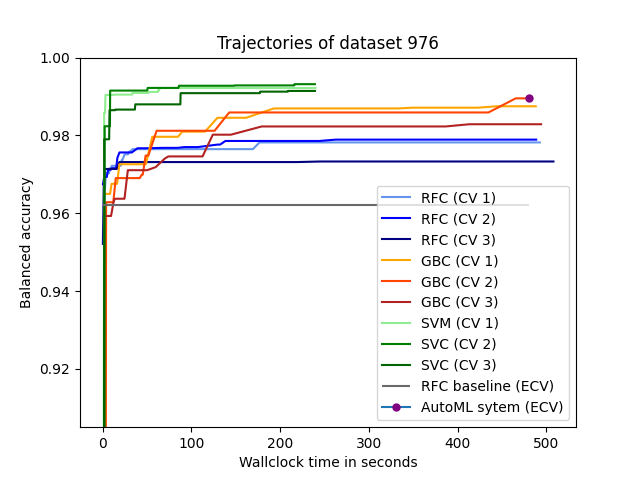
\includegraphics[width=0.75\textwidth]{fig/plot_dataset_976.png}
  \caption{Trajectories for dataset 976 with 9961 observations and 14 features.}
\end{figure}

\begin{figure}[H]
 \centering
  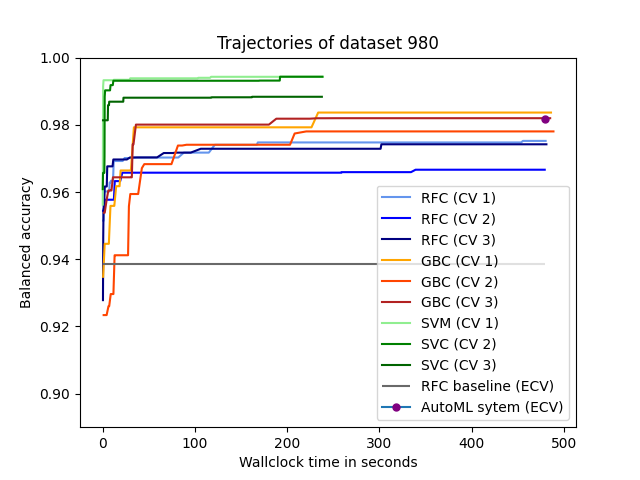
\includegraphics[width=0.75\textwidth]{fig/plot_dataset_980.png}
  \caption{Trajectories for dataset 980 with 5620 observations and 64 features.}
\end{figure}

\begin{figure}[H]
 \centering
  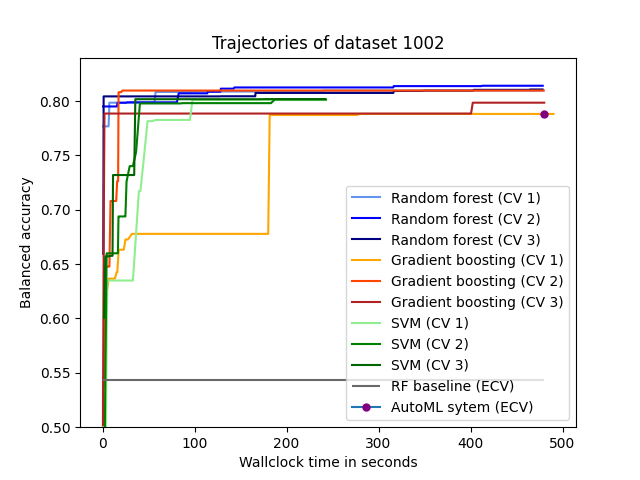
\includegraphics[width=0.75\textwidth]{fig/plot_dataset_1002.png}
  \caption{Trajectories for dataset 1002 with 7485 observations and 55 features.}
\end{figure}

\begin{figure}[H]
 \centering
  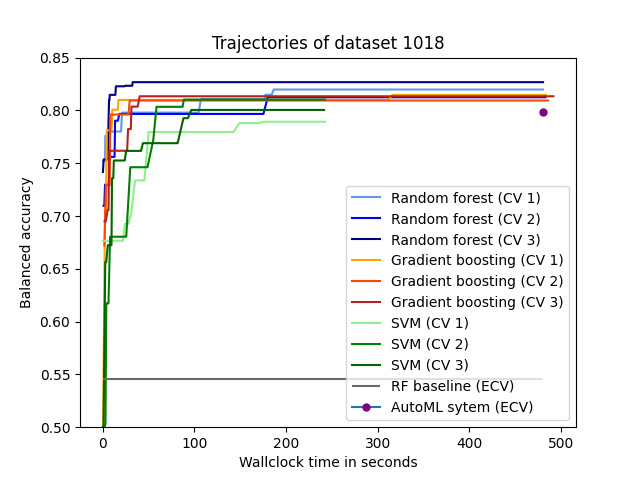
\includegraphics[width=0.75\textwidth]{fig/plot_dataset_1018.png}
  \caption{Trajectories for dataset 1018 with 8844 observations and 56 features.}
\end{figure}

\begin{figure}[H]
 \centering
  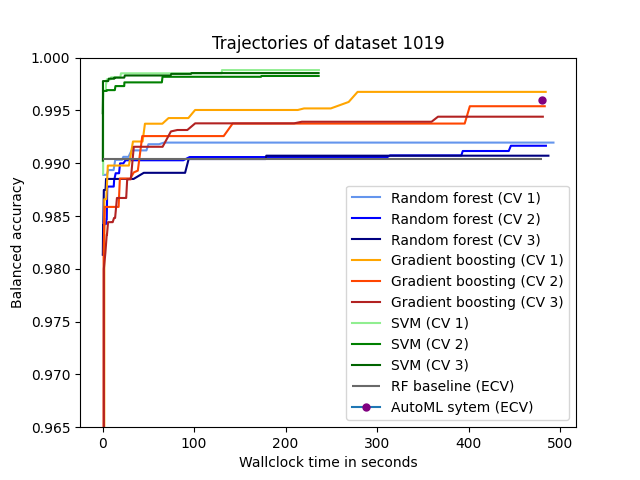
\includegraphics[width=0.75\textwidth]{fig/plot_dataset_1019.png}
  \caption{Trajectories for dataset 1019 with 10992 observations with 16 features}
\end{figure}

\begin{figure}[H]
 \centering
  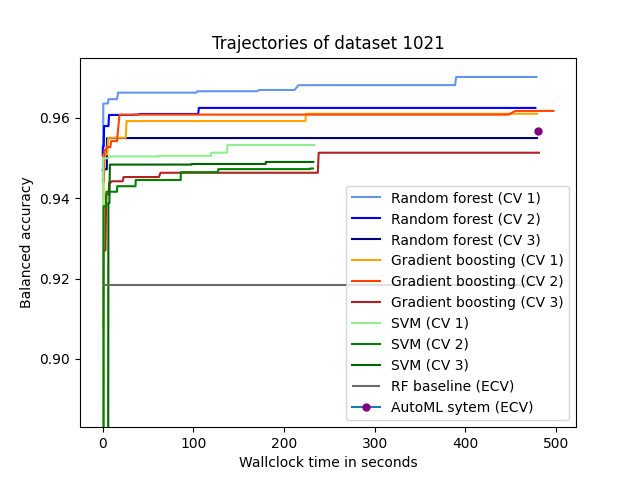
\includegraphics[width=0.75\textwidth]{fig/plot_dataset_1021.png}
  \caption{Trajectories for dataset 1021 with 5473 observations and 10 features.}
\end{figure}

\begin{figure}[H]
 \centering
  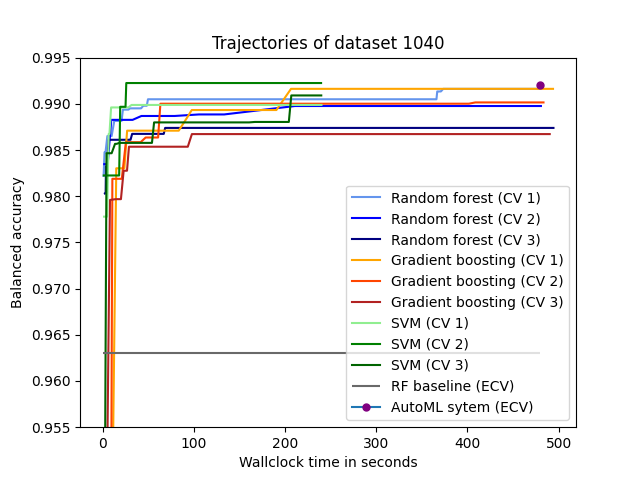
\includegraphics[width=0.75\textwidth]{fig/plot_dataset_1040.png}
  \caption{Trajectories for dataset 1040 with 14395 observations and 108 features.}
\end{figure}

\begin{figure}[H]
 \centering
  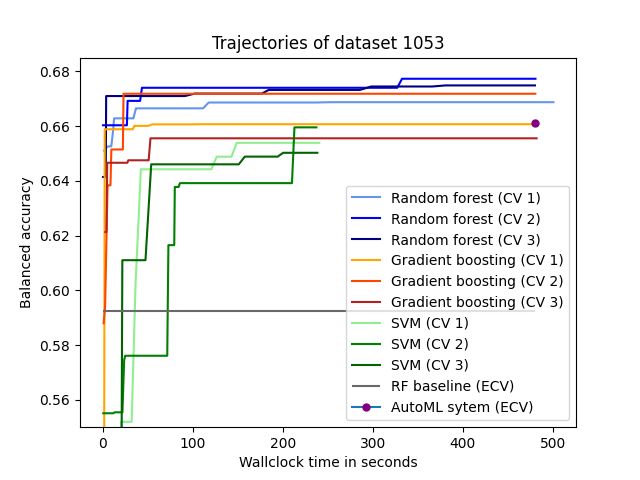
\includegraphics[width=0.75\textwidth]{fig/plot_dataset_1053.png}
  \caption{Trajectories for dataset 1053 with 10885 observations and 21 features.}
\end{figure}

\begin{figure}[H]
 \centering
  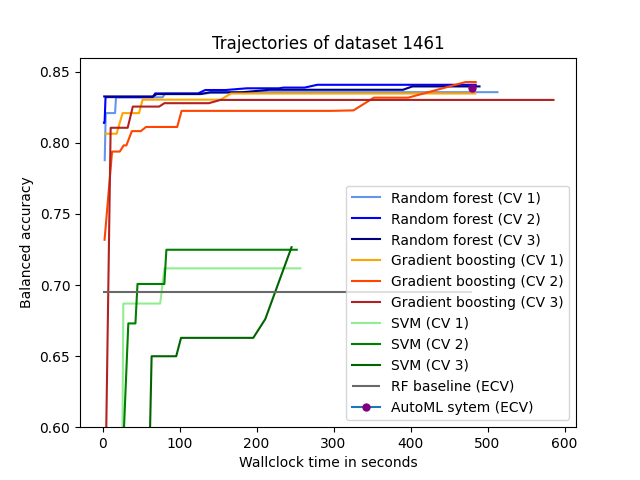
\includegraphics[width=0.75\textwidth]{fig/plot_dataset_1461.png}
  \caption{Trajectories for dataset 1461 with 45221 observations and 16 features.}
\end{figure}

\begin{figure}[H]
 \centering
  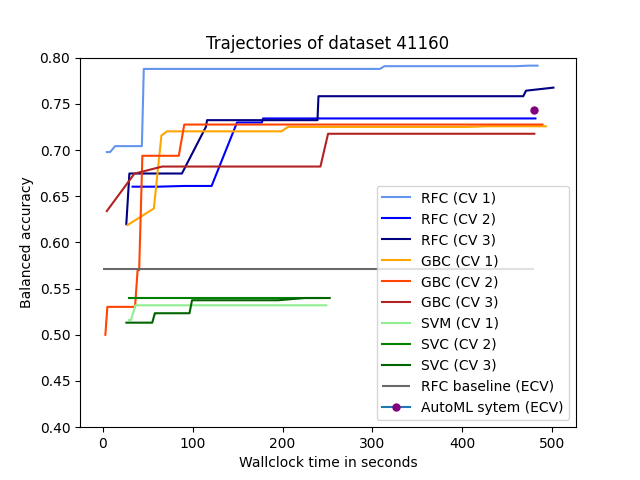
\includegraphics[width=0.75\textwidth]{fig/plot_dataset_41160.png}
  \caption{Trajectories for dataset 41660 with 31406 observations and 22 features.}
\end{figure}

\section{Incumbent hyperparameter}

The following tables shows the incumbent hyperparameter configurations for each algorithm and each dataset in each fold. 

\begin{sidewaystable}
\footnotesize
\caption{Incumbent hyperparameter configurations for the random forest classifier}
\center
\begin{tabularx}{22cm}{lllllllXXXX}
\toprule
Dataset ID & CV fold & Imputer &    Sampler & Scaler & Criterion & Max depth & Min samples \newline per split & Min samples \newline per leaf &  Max features &       Class weight \\
\midrule
       976 &       1 &  Simple & SMOTETomek &  False &   entropy &        22 &                     4 &                    1 &      0.656466 &               None \\
       976 &       2 &  Simple & SMOTETomek &   True &  log\_loss &        17 &                     4 &                    1 &      0.115289 & balanced\_subsample \\
       976 &       3 &  Simple &      SMOTE &  False &   entropy &        16 &                     4 &                    2 &      0.262840 &           balanced \\
\midrule
       980 &       1 &  Simple & SMOTETomek &  False &   entropy &        16 &                     2 &                    2 &      0.457415 &               None \\
       980 &       2 &     KNN & SMOTETomek &   True &   entropy &        19 &                     2 &                    9 &      0.282039 &           balanced \\
       980 &       3 &  Simple & SMOTETomek &   True &  log\_loss &        11 &                     1 &                    6 &      0.144065 &               None \\
\midrule
      1002 &       1 &     KNN &      Tomek &  False &   entropy &         5 &                     8 &                    2 &      0.228523 & balanced\_subsample \\
      1002 &       2 &  Simple &       None &  False &  log\_loss &         5 &                     5 &                    9 &      0.392731 & balanced\_subsample \\
      1002 &       3 &  Simple &      Tomek &   True &      gini &         6 &                    11 &                    4 &      0.192183 &           balanced \\
\midrule
      1018 &       1 &     KNN &      Tomek &  False &   entropy &         6 &                     1 &                   14 &      0.105286 &           balanced \\
      1018 &       2 &     KNN &      Tomek &  False &  log\_loss &         5 &                    25 &                    3 &      0.497648 & balanced\_subsample \\
      1018 &       3 &     KNN &      Tomek &   True &      gini &         5 &                     9 &                    6 &      0.285309 &           balanced \\
\midrule
      1019 &       1 &  Simple & SMOTETomek &   True &   entropy &        23 &                     2 &                    1 &      0.806836 & balanced\_subsample \\
      1019 &       2 &     KNN & SMOTETomek &  False &   entropy &        19 &                     3 &                    1 &      0.195487 &               None \\
      1019 &       3 &  Simple &      SMOTE &   True &  log\_loss &        24 &                     1 &                    5 &      0.726165 &               None \\
\midrule
      1021 &       1 &     KNN &      SMOTE &  False &      gini &        20 &                    19 &                    4 &      0.134323 & balanced\_subsample \\
      1021 &       2 &  Simple &      SMOTE &  False &   entropy &        22 &                     9 &                    9 &      0.495168 &           balanced \\
      1021 &       3 &  Simple & SMOTETomek &   True &   entropy &        24 &                    14 &                    3 &      0.208502 &               None \\
\midrule
      1040 &       1 &  Simple & SMOTETomek &  False &      gini &         8 &                    11 &                    4 &      0.577811 & balanced\_subsample \\
      1040 &       2 &  Simple & SMOTETomek &  False &      gini &        23 &                     2 &                    5 &      0.797167 &               None \\
      1040 &       3 &     KNN &      Tomek &  False &      gini &         5 &                     1 &                    1 &      0.390420 &           balanced \\
\midrule
      1053 &       1 &     KNN & SMOTETomek &  False &  log\_loss &         9 &                     2 &                    4 &      0.393722 & balanced\_subsample \\
      1053 &       2 &     KNN &      Tomek &   True &  log\_loss &         7 &                     9 &                    4 &      0.791928 &           balanced \\
      1053 &       3 &  Simple &      Tomek &   True &   entropy &        18 &                     4 &                   12 &      0.656912 & balanced\_subsample \\
\midrule
      1461 &       1 &     KNN &      Tomek &  False &  log\_loss &        20 &                     1 &                   11 &      0.158737 & balanced\_subsample \\
      1461 &       2 &     KNN & SMOTETomek &   True &   entropy &        11 &                    21 &                    4 &      0.517657 &           balanced \\
      1461 &       3 &     KNN &      Tomek &  False &   entropy &        14 &                    31 &                    2 &      0.221436 &           balanced \\
\midrule
     41160 &       1 &  Simple &       None &  False &   entropy &        18 &                     4 &                    6 &      0.769477 &           balanced \\
     41160 &       2 &  Simple &      Tomek &   True &   entropy &        10 &                    28 &                    3 &      0.783361 &           balanced \\
     41160 &       3 &  Simple &      Tomek &   True &      gini &        12 &                     3 &                    4 &      0.808427 &           balanced \\
\bottomrule
\end{tabularx}
\end{sidewaystable}


\begin{sidewaystable}
\footnotesize
\caption{Incumbent hyperparameter configurations for the gradient boosting classifier}
\center
\begin{tabular}{lllllllllll}
\toprule
Dataset ID & CV fold & Imputer &    Sampler & Scaler &        Loss &  Learning rate &     Criterion & Min samples per split & Min samples per leaf & Max depth \\
\midrule
       976 &       1 &  Simple &      SMOTE &   True & exponential &       0.814630 &  friedman\_mse &                     3 &                    2 &         8 \\
       976 &       2 &  Simple & SMOTETomek &   True & exponential &       0.979669 &  friedman\_mse &                     6 &                    8 &        10 \\
       976 &       3 &     KNN & SMOTETomek &  False & exponential &       0.948759 &  friedman\_mse &                     4 &                   11 &         8 \\
\midrule
       980 &       1 &  Simple &      SMOTE &   True &    log\_loss &       0.360042 &  friedman\_mse &                     4 &                    9 &         4 \\
       980 &       2 &     KNN & SMOTETomek &   True & exponential &       0.359648 & squared\_error &                    10 &                    1 &         4 \\
       980 &       3 &     KNN & SMOTETomek &   True & exponential &       0.366579 & squared\_error &                    24 &                   12 &         4 \\
\midrule
      1002 &       1 &     KNN & SMOTETomek &   True & exponential &       0.023344 &  friedman\_mse &                     5 &                    1 &         3 \\
      1002 &       2 &     KNN &      SMOTE &   True &    log\_loss &       0.016664 &  friedman\_mse &                     2 &                    5 &         2 \\
      1002 &       3 &  Simple & SMOTETomek &   True &    log\_loss &       0.026060 &  friedman\_mse &                     4 &                    3 &         3 \\
\midrule
      1018 &       1 &  Simple &      SMOTE &   True & exponential &       0.039226 &  friedman\_mse &                     9 &                   13 &         2 \\
      1018 &       2 &  Simple & SMOTETomek &  False & exponential &       0.027759 & squared\_error &                    21 &                    1 &         4 \\
      1018 &       3 &     KNN &      SMOTE &  False &    log\_loss &       0.065935 &  friedman\_mse &                    13 &                    6 &         3 \\
\midrule
      1019 &       1 &     KNN & SMOTETomek &   True & exponential &       0.566058 &  friedman\_mse &                    11 &                    5 &         4 \\
      1019 &       2 &     KNN &      SMOTE &   True & exponential &       0.686387 & squared\_error &                    10 &                    1 &         6 \\
      1019 &       3 &  Simple & SMOTETomek &   True &    log\_loss &       0.358116 & squared\_error &                     7 &                    2 &         4 \\
\midrule
      1021 &       1 &  Simple &      SMOTE &   True &    log\_loss &       0.230746 &  friedman\_mse &                    24 &                    8 &         5 \\
      1021 &       2 &  Simple &      SMOTE &  False & exponential &       0.020508 &  friedman\_mse &                    12 &                    6 &        11 \\
      1021 &       3 &     KNN & SMOTETomek &  False &    log\_loss &       0.283118 & squared\_error &                     5 &                    2 &         3 \\
\midrule
      1040 &       1 &  Simple &      SMOTE &   True & exponential &       0.428100 &  friedman\_mse &                    14 &                    1 &         3 \\
      1040 &       2 &     KNN &      SMOTE &   True & exponential &       0.690849 &  friedman\_mse &                    11 &                    4 &         4 \\
      1040 &       3 &     KNN & SMOTETomek &   True & exponential &       0.545570 &  friedman\_mse &                     5 &                    5 &         2 \\
\midrule
      1053 &       1 &  Simple & SMOTETomek &   True & exponential &       0.031338 &  friedman\_mse &                     3 &                   10 &         5 \\
      1053 &       2 &  Simple &      SMOTE &   True &    log\_loss &       0.010315 &  friedman\_mse &                     8 &                    8 &         2 \\
      1053 &       3 &  Simple & SMOTETomek &  False & exponential &       0.038175 &  friedman\_mse &                     5 &                    6 &         2 \\
\midrule
      1461 &       1 &     KNN & SMOTETomek &  False & exponential &       0.097863 &  friedman\_mse &                     3 &                    4 &         5 \\
      1461 &       2 &     KNN & SMOTETomek &   True & exponential &       0.129724 &  friedman\_mse &                    23 &                    4 &         7 \\
      1461 &       3 &     KNN &      SMOTE &   True & exponential &       0.092295 & squared\_error &                    26 &                   14 &         6 \\
\midrule
     41160 &       1 &     KNN &      SMOTE &  False &    log\_loss &       0.018754 &  friedman\_mse &                     4 &                   11 &        14 \\
     41160 &       2 &  Simple & SMOTETomek &  False &    log\_loss &       0.025380 &  friedman\_mse &                     5 &                    2 &         8 \\
     41160 &       3 &  Simple &      SMOTE &  False & exponential &       0.011618 & squared\_error &                     5 &                   16 &        10 \\
\bottomrule
\end{tabular}
\end{sidewaystable}

\begin{sidewaystable}
\footnotesize
\caption{Incumbent hyperparameter configurations for the SVM classifier}
\center
\begin{tabular}{llllllllll}
\toprule
Dataset ID & CV fold & Imputer &    Sampler & Scaler &        C &  Kernel & Shrinking &  Tolerance & Class weight \\
\midrule
       976 &       1 &     KNN &       None &   True & 6.812195 &     rbf &      True & 0.000136 &     balanced \\
       976 &       2 &  Simple & SMOTETomek &   True & 5.942369 &     rbf &      True & 0.002453 &     balanced \\
       976 &       3 &  Simple &      Tomek &   True & 5.042524 &     rbf &     False & 0.000554 &     balanced \\
\midrule
       980 &       1 &  Simple & SMOTETomek &   True & 2.461050 &    poly &     False & 0.004004 &     balanced \\
       980 &       2 &  Simple &      SMOTE &   True & 0.810882 &    poly &      True & 0.002291 &     balanced \\
       980 &       3 &     KNN &      Tomek &  False & 1.221203 &     rbf &     False & 0.003969 &     balanced \\
\midrule
      1002 &       1 &     KNN &      Tomek &   True & 0.230800 &  linear &     False & 0.002982 &     balanced \\
      1002 &       2 &     KNN & SMOTETomek &   True & 0.127835 & sigmoid &      True & 0.001461 &     balanced \\
      1002 &       3 &  Simple & SMOTETomek &   True & 0.384752 &  linear &     False & 0.005138 &     balanced \\
\midrule
      1018 &       1 &  Simple &      SMOTE &   True & 0.202185 & sigmoid &     False & 0.000893 &         None \\
      1018 &       2 &  Simple &       None &   True & 0.245091 &  linear &      True & 0.001234 &     balanced \\
      1018 &       3 &  Simple & SMOTETomek &   True & 0.135464 &  linear &     False & 0.000205 &     balanced \\
\midrule
      1019 &       1 &     KNN &      Tomek &  False & 9.389382 &    poly &     False & 0.000422 &         None \\
      1019 &       2 &     KNN & SMOTETomek &  False & 1.538617 &    poly &     False & 0.000794 &         None \\
      1019 &       3 &     KNN & SMOTETomek &  False & 9.673782 &     rbf &      True & 0.002117 &     balanced \\
\midrule
      1021 &       1 &     KNN &       None &   True & 7.955140 &     rbf &     False & 0.000758 &     balanced \\
      1021 &       2 &     KNN &       None &   True & 8.527953 &     rbf &     False & 0.000206 &     balanced \\
      1021 &       3 &     KNN &      Tomek &   True & 7.187957 &     rbf &      True & 0.000581 &     balanced \\
\midrule
      1040 &       1 &  Simple & SMOTETomek &   True & 0.506277 &  linear &      True & 0.001319 &         None \\
      1040 &       2 &     KNN &      Tomek &   True & 0.126113 &  linear &     False & 0.003028 &     balanced \\
      1040 &       3 &  Simple & SMOTETomek &   True & 1.165825 & sigmoid &      True & 0.002011 &         None \\
\midrule
      1053 &       1 &  Simple & SMOTETomek &   True & 2.294233 &     rbf &     False & 0.000396 &         None \\
      1053 &       2 &  Simple &      Tomek &   True & 3.810805 &     rbf &     False & 0.009082 &     balanced \\
      1053 &       3 &     KNN & SMOTETomek &   True & 1.594506 &  linear &     False & 0.001114 &     balanced \\
\midrule
      1461 &       1 &  Simple & SMOTETomek &   True & 0.485222 & sigmoid &     False & 0.000393 &         None \\
      1461 &       2 &  Simple &      Tomek &   True & 3.769543 & sigmoid &      True & 0.001322 &     balanced \\
      1461 &       3 &  Simple &       None &   True & 0.533370 & sigmoid &     False & 0.008771 &     balanced \\
\midrule
     41160 &       1 &     KNN &      Tomek &   True & 8.007605 &     rbf &     False & 0.000958 &         None \\
     41160 &       2 &     KNN &      SMOTE &   True & 0.227120 &     rbf &      True & 0.001452 &     balanced \\
     41160 &       3 &  Simple &      SMOTE &   True & 9.758566 & sigmoid &     False & 0.000217 &     balanced \\
\bottomrule
\end{tabular}
\end{sidewaystable}

\section{Information about datasets}

\center
\begin{tabular}{llllllllll}
\toprule
Dataset ID & Observations & Features \\
\midrule
976 & 9961 & 14 \\
980 & 5620 & 64 \\
1002 & 7485 & 55 \\
1018 & 8844 & 56 \\
1019 & 10992 & 16 \\
1021 & 5473 & 10 \\
1040 & 14395 & 108 \\
1053 & 10885 & 21 \\
1461 & 45221 & 16 \\
41160 & 31406 & 22 \\
\bottomrule
\end{tabular}

% complete 

\end{document}
